% !TEX root = ../main.tex
\chapter{绪论}
\label{chap01}

长久以来,人们对于自然界中存在的物质的基本组成一直充满了好奇，无数科学家在对自然科学的规律进行探索的时候，无不例外的都会关注同一个问题：物质的最小组成单位是什么？
从古代人们通过直觉对事物的朴素认知，再到二十世纪初的基本粒子理论，科学家们对于物质基本组成单位的认识经历了一个不断深化的过程。而从某种程度上来说，粒子物理学的发展可以按照各个基本粒子的发现来展开。\\

1897年，约瑟夫·汤姆逊在电磁场中通过带电粒子束测量了电子的荷质比，
1911年，欧内斯特·卢瑟福及其助手进行了著名的金箔 $\alpha$ 粒子散射实验。他们用带正电的 $\alpha$ 粒子轰击极薄的金箔，发现绝大多数粒子径直穿过，但有极少数粒子发生了大角度偏转，甚至原路反弹。
基于这一反常现象，卢瑟福推翻了汤姆逊的“枣糕模型”，提出了原子的“核式结构模型”：原子内部极其空旷，原子的中心存在一个体积极小、却集中了所有正电荷和几乎全部质量的“原子核”，而电子则在核外的广阔空间绕核运动。
1932年，詹姆斯·查德威克在用 $\alpha$ 粒子轰击金属铍靶的核反应实验中，产生了一种穿透力极强的中性辐射。查德威克利用这种射线轰击氢、氮等物质，通过测量反冲核的动量和能量，证实这种射线是一种质量与质子极其相近、但不带电的中性微粒，即“中子”。
中子的发现补全了原子核由质子和中子组成的现代模型。\\

到了20世纪50年代，随着现代高能粒子加速器的相继建成与运行，物理学家们能够在更高的能量尺度下让粒子发生剧烈碰撞。
在这一时期，实验中发现了一大批前所未见的新粒子以及寿命极短的共振态，
例如超子（如 $\Lambda$、$\Sigma$、$\Xi$ 粒子）和各种介子。这些层出不穷的粒子为后来提出“夸克模型”以及建立粒子物理标准模型奠定了实验基础。

%%%%%%%%%%%%%%%%%%%%%%%%%%%%基本粒子总表%%%%%%%%%%%%%%%%%%%%%%%%%%%%%
\begin{table}[htbp]
\centering
\small
\setlength{\tabcolsep}{7pt}
\renewcommand{\arraystretch}{1.15}
\caption{标准模型基本粒子内容概览（按代与相互作用分类）。}
\label{tab:SM_overview_noRemark}

\resizebox{\linewidth}{!}{%
\begin{tabular}{llll}
\toprule
类别 & 子类 & 记号 & 电荷 $Q$ \\
\midrule
\multirow{3}{*}{费米子（物质粒子）}
& 第1代 & $(\nu_e,\,e^-);\ (u,\,d)$ & $0,\,-1;\ \frac{2}{3},\,-\frac{1}{3}$ \\
& 第2代 & $(\nu_\mu,\,\mu^-);\ (c,\,s)$ & $0,\,-1;\ \frac{2}{3},\,-\frac{1}{3}$ \\
& 第3代 & $(\nu_\tau,\,\tau^-);\ (t,\,b)$ & $0,\,-1;\ \frac{2}{3},\,-\frac{1}{3}$ \\
\midrule
\multirow{3}{*}{规范玻色子（相互作用媒介）}
& 强相互作用 & $g^a\ (a=1,\dots,8)$ & $0$ \\
& 电磁相互作用 & $\gamma$ & $0$ \\
& 弱相互作用 & $W^\pm,\ Z^0$ & $\pm 1,\ 0$ \\
\midrule
标量玻色子 & 希格斯 & $H$ & $0$ \\
\bottomrule
\end{tabular}%
}
\end{table}

\section{标准模型与基本粒子的分类}

标准模型（Standard Model, SM）是目前描述微观世界中基本粒子及其相互作用最成功的理论框架。该理论建立在规范场论的基础之上，其基本对称性由如下规范群决定：
\begin{equation}
SU(3)_C \times SU(2)_L \times U(1)_Y ,
\end{equation}
分别对应强相互作用、电弱相互作用中的弱同位旋对称性以及弱超荷对称性。\\

在标准模型中，自然界的基本相互作用（除引力外）均可由规范场交换来描述：由量子色动力学(QCD)描述的强相互作用、由量子电动力学（QED）描述的电磁相互作用，以及由电弱理论描述的弱相互作用。
标准模型中的基本组成单元包括传递相互作用的规范玻色子、构成物质的费米子、以及产生粒子质量的希格斯粒子。根据自旋统计定理，费米子具有半整数自旋，而玻色子具有整数自旋。\\

对于规范玻色子，强相互作用由八种胶子（$g$）传递，电磁相互作用由光子（$\gamma$）传递，而弱相互作用则由 $W^\pm$ 和 $Z^0$ 玻色子传递。它们的都具有相同的为$1$的自旋，但质量不同，光子无质量，$W^\pm$ 和 $Z^0$ 具有较大的质量。一共有$1+3+8=12$个规范玻色子。
对于费米子而言，现在人们已知至少存在三代费米子，每一代包括两个两个轻子，考虑到每个轻子的反粒子，总计是$12$个轻子，而对于$6$种不同味道的夸克，考虑到其反粒子共 $12$ 种,每个夸克还有三种不同的颜色，所以总计共$36$个带色的夸克态。
我们知道，在费米子中，轻子和夸克的自旋都是$1/2$，而规范场要求所有费米子的电荷之和为零，所以轻子和夸克总是成代的出现，每一代的电荷之和都为零，这也是标准模型中一个重要的特征。
对于希格斯粒子，它的自旋为$0$，负责通过自发对称性破缺机制赋予其他粒子质量。希格斯粒子的发现是标准模型的一个重要里程碑，验证了该机制的正确性。
% 按照现有的理论体系，标准模型中包括的基本粒子数量为$12+(6+6)+(6\times3\times2)+ 1$，按照质量与味结构可分为三代（three generations）。这些基本粒子共同组成了数百种各式各样的复合粒子（如质子、中子、介子等），并通过各种相互作用构成了我们所观察到的物质世界。\\
按照现有的理论体系，标准模型中包括的基本粒子数量为 $12+(6+6)+(6\times3\times2)+ 1$，按照质量与味结构可分为三代。具体而言，这一粒子谱包含了 $12$ 个传递基本相互作用的规范玻色子、$12$ 个轻子（含反粒子）、$36$ 个携带色荷的夸克（含反夸克与三种色态），以及 $1$ 个负责电弱对称性破缺并赋予基本费米子质量的标量希格斯玻色子。其中，自然界最稳定的可见物质主要由第一代费米子（如 $u$ 夸克、$d$ 夸克与电子）构成，而更高代的重粒子通常极不稳定，仅在宇宙早期或高能对撞实验中短暂存在。这些基本粒子共同组成了数百种各式各样的复合粒子（如基态的质子、中子以及大量介子和重子共振态），并通过定域规范群 $\mathrm{SU}(3)_c \otimes \mathrm{SU}(2)_L \otimes \mathrm{U}(1)_Y$ 所支配的强、弱及电磁相互作用，构成了我们所观察到的宏观与微观物质世界。\\

%%%%%%%%%%%%%%%%%%%%%%%%%%%%%%%%%%%%%%%%%夸克和轻子的代%%%%%%%%%%%%%%%%%%%%%%%%%%%%%%

\begin{table}[!htb]
\centering
\small
\setlength{\tabcolsep}{10pt}
\renewcommand{\arraystretch}{1.25}
\caption{夸克和轻子的代结构（按电荷类型与代排列）。}
\label{tab:gen_quark_lepton}

\resizebox{\linewidth}{!}{%
\begin{tabular}{c|ccc}
\toprule
类 & 第一代 & 第二代 & 第三代 \\
\midrule
\multicolumn{4}{c}{\textbf{夸克}} \\
\midrule
上型（$Q=+\frac{2}{3}$） & 上夸克（up, $u$） & 粲夸克（charm, $c$） & 顶夸克（top, $t$） \\
下型（$Q=-\frac{1}{3}$） & 下夸克（down, $d$） & 奇夸克（strange, $s$） & 底夸克（bottom, $b$） \\
\midrule
\multicolumn{4}{c}{\textbf{轻子}} \\
\midrule
带电（$Q=-1$） & 电子（$e^-$） & $\mu$子（$\mu^-$） & $\tau$子（$\tau^-$） \\
中性（$Q=0$） & 电子中微子（$\nu_e$） & $\mu$子中微子（$\nu_\mu$） & $\tau$子中微子（$\nu_\tau$） \\
\bottomrule
\end{tabular}%
}
\end{table}

%%%%%%%%%%%%%%%%%%%%%%%%%%%%%%%夸克的量子数%%%%%%%%%%%%%%%%%%%%%%%%%%%%%%%%%%%
\begin{table}[!htb]
\centering
\renewcommand{\arraystretch}{1.3}
\setlength{\tabcolsep}{12pt}
\caption{夸克的量子数。}
\label{tab:quark_quantum_numbers}

\resizebox{\linewidth}{!}{%
\begin{tabular}{c c c c c c c c}
\toprule
味道 & $Q$ & $I$ & $I_z$ & $S$ & $C$ & $B$ & $T$ \\
\midrule
$u$ & $+\frac{2}{3}$ & $\frac{1}{2}$ & $+\frac{1}{2}$ & $0$  & $0$  & $0$  & $0$ \\
$d$ & $-\frac{1}{3}$ & $\frac{1}{2}$ & $-\frac{1}{2}$ & $0$  & $0$  & $0$  & $0$ \\
$s$ & $-\frac{1}{3}$ & $0$           & $0$            & $-1$ & $0$  & $0$  & $0$ \\
$c$ & $+\frac{2}{3}$ & $0$           & $0$            & $0$  & $+1$ & $0$  & $0$ \\
$b$ & $-\frac{1}{3}$ & $0$           & $0$            & $0$  & $0$  & $-1$ & $0$ \\
$t$ & $+\frac{2}{3}$ & $0$           & $0$            & $0$  & $0$  & $0$  & $+1$ \\
\bottomrule
\end{tabular}%
}
\end{table}

\section{强子结构模型}

作为描述强相互作用的基本规范场论，量子色动力学（QCD）建立在非阿贝尔定域规范对称性 $\mathrm{SU}(3)_c$ 的基础之上。在该理论框架内，夸克作为构成强子的基本费米子，处于 $\mathrm{SU}(3)_c$ 群的基本表示，并携带被称为“色”的量子数。传递强相互作用的规范玻色子是胶子，处于伴随表示，由8个无质量的非阿贝尔规范场描述。由于规范群的非阿贝尔性质，胶子自身也携带色荷，这使得胶子之间存在自相互作用。这种非线性的动力学机制是导致 QCD 在高能区呈现渐近自由、在低能区主导非微扰现象的根本原因。
在低能非微扰 QCD 图像中，一个核心特征是色禁闭机制。该机制指出，携带色荷的裸夸克和胶子无法在自然界中作为自由粒子被分离出来；所有在实验中可被直接观测到的渐近物理态即强子态，必须是由夸克和胶子组成的 $\mathrm{SU}(3)_c$ 色单态。\\

由于胶子仅携带色荷而具有零味量子数，强子的宏观量子数（如电荷、同位旋、奇异数等）完全由其内部价夸克与反夸克的组分所决定。根据自旋统计定理与狄拉克方程，夸克是自旋为 $1/2$ 且内禀宇称为正（$P=+1$）的费米子，相应的反夸克则具有负的内禀宇称（$P=-1$）。迄今为止，标准模型在实验上共确认了六种具有不同味道的夸克，按质量排列分为三代：上（$u$）、下（$d$）、奇异（$s$）、粲（$c$）、底（$b$）以及顶（$t$）夸克。这些不同味道的夸克通过结合成各种色单态结构，构成了自然界中极其丰富的强子能谱。\\

在传统意义上的夸克模型中，强子被认为是由夸克和反夸克组成的复合粒子。盖尔曼于1961年根据奇异数守恒，用$SU(3)$对称性将基本粒子进行分类，盖尔曼认为，强子是由夸克和反夸克组成的复合粒子，其中$u、d、s$夸克质量较轻，被称为轻夸克，$c、b、t$夸克质量较重，被称为重夸克。
夸克具有分数电荷和色荷。根据盖尔曼——西岛关系，夸克的量子数有着以下关系
\vspace{0.5cm}
\begin{equation}
    Q = I_3 + \frac{Y}{2} = I_3 + \frac{b+S+C+B+T}{2} ,
\end{equation}

其中$Q$是电荷，$I_3$是同位旋第三分量，$Y$是超荷，$b$是重子数，$S$是奇异数，$C$是粲数，$B$是底数。
根据夸克的组合方式，强子可以分为两大类：介子（Mesons）和重子（Baryons）。
介子是由一个夸克和一个反夸克通过胶子的连接组成的强子，具有整数自旋，因此是玻色子。例如，$\pi$介子（由$u\bar{d}$或$d\bar{u}$组成）和$K$介子（由$s\bar{u}$或$s\bar{d}$组成）都是常见的介子。
重子则是由三个夸克组成的强子，具有半整数自旋，因此是费米子。例如，质子（由$uud$组成）和中子（由$udd$组成）是最常见的重子。

\subsection{介子}
介子可以按照角动量$J$，$P$宇称和$C$宇称进行分类，在一个介子系统中，角动量$J$的范围是， $|l-s|\leq J \leq l+s$，其中$L$是轨道角动量，$S$是自旋。对于介子系统，宇称$P=(-1)^{l+1}$，电中性介子的C宇称为$C=(-1)^{l+s}$。
于是介子便可以按照$J^{PC}$进行分类。当系统角动量$J=0$时，介子被称为标量介子；当系统角动量$J=1$时，介子被称为矢量介子；当系统角动量$J=2$时，介子被称为张量介子。如果我们仅仅考虑由$u$、$d$、$s$三种轻夸克组成的介子系统，那么我们可以按照其味道进行分类，形成一个八重态和一个单态。
根据$SU(3)_F$对称性，基态赝标介子（$0^{-+}$）八重态包括$\pi$介子（$u\bar{d}$、$d\bar{u}$、$u\bar{u}-d\bar{d}$）、$K$介子（$s\bar{u}$、$s\bar{d}$、$u\bar{s}$、$d\bar{s}$）和$\eta$介子（$u\bar{u}+d\bar{d}-2s\bar{s}$），而单态则是$\eta'$介子。
同理，基态矢量介子（$1^{--}$）八重态包括$\rho$介子（$u\bar{d}$、$d\bar{u}$、$u\bar{u}-d\bar{d}$）、$K^*$介子（$s\bar{u}$、$s\bar{d}$、$u\bar{s}$、$d\bar{s}$）和$\omega$介子（$u\bar{u}+d\bar{d}$），而单态则是$\phi$介子。赝标介子和矢量介子八重态权图如下图所示。\\


\begin{figure}[htbp]
\centering

% 统一样式：白底遮罩
\tikzset{
  ticklab/.style={font=\scriptsize, fill=white, inner sep=1.2pt},
  plab/.style={fill=white, inner sep=1.2pt},
  axlab/.style={fill=white, inner sep=1.2pt}
}

%==================== 左：赝标介子八重态 ====================
\begin{minipage}{0.46\textwidth}
\centering
\resizebox{\linewidth}{!}{%
\begin{tikzpicture}[x=2.25cm,y=1.85cm, line cap=round, line join=round]

% 坐标轴
\draw[->,thick] (-1.28,0) -- (1.28,0) node[axlab,below right=2pt] {$I_3$};
\draw[->,thick] (0,-1.28) -- (0,1.28) node[axlab,above left=2pt] {$Y$};

% 点坐标
\coordinate (pi-) at (-1,0);
\coordinate (pi+) at ( 1,0);
\coordinate (K0)  at (-0.5, 1);
\coordinate (K+)  at ( 0.5, 1);
\coordinate (Km)  at (-0.5,-1);
\coordinate (K0b) at ( 0.5,-1);
\coordinate (C)   at (0,0);

% 六边形
\draw[thick] (pi-) -- (K0) -- (K+) -- (pi+) -- (K0b) -- (Km) -- cycle;

% 黑点
\foreach \p in {pi-,pi+,K0,K+,Km,K0b,C}
  \fill (\p) circle (1.8pt);

% 粒子标注
\node[plab,above=1.5pt]      at (pi-) {$\pi^-$};
\node[plab,above=1.5pt]      at (pi+) {$\pi^+$};

\node[plab,above left=1.5pt] at (K0)  {$K^0$};
\node[plab,above right=1.5pt]at (K+)  {$K^+$};

\node[plab,below=1.5pt]      at (Km)  {$K^-$};
\node[plab,below=1.5pt]      at (K0b) {$\overline{K}{}^{0}$};

\node[plab,above=1.5pt] at ($(C)+(-0.10,0)$) {$\pi^0$};
\node[plab,above=1.5pt] at ($(C)+( 0.10,0)$) {$\eta_8$};

% 虚线
\draw[dashed] (-0.5,0) -- (-0.5,1);

% 刻度线
\foreach \x in {-1,-0.5,0,0.5,1}{
  \draw[thick] (\x,0) -- (\x,0.035);
}
\foreach \y in {-1,0,1}{
  \draw[thick] (0,\y) -- (0.035,\y);
}

% x轴刻度数字
\node[ticklab,below=3pt] at (-1,0)   {$-1$};
\node[ticklab,below=3pt] at (-0.5,0) {$-1/2$};
\node[ticklab,below=3pt] at ( 0.5,0) {$1/2$};
\node[ticklab,below=3pt] at ( 1,0)   {$1$};

% y轴刻度数字
\node[ticklab,right=3.5pt] at (0, 1) {$1$};
\node[ticklab,right=3.5pt] at (0,-1) {$-1$};

% 原点
\node[ticklab,below right=2pt] at (0,0) {$0$};

\end{tikzpicture}%
}
\end{minipage}
\hfill
%==================== 右：矢量介子八重态 ====================
\begin{minipage}{0.46\textwidth}
\centering
\resizebox{\linewidth}{!}{%
\begin{tikzpicture}[x=2.25cm,y=1.85cm, line cap=round, line join=round]

% 坐标轴
\draw[->,thick] (-1.28,0) -- (1.28,0) node[axlab,below right=2pt] {$I_3$};
\draw[->,thick] (0,-1.28) -- (0,1.28) node[axlab,above left=2pt] {$Y$};

% 点坐标
\coordinate (rho-) at (-1,0);
\coordinate (rho+) at ( 1,0);
\coordinate (Kst0)  at (-0.5, 1);
\coordinate (Kst+)  at ( 0.5, 1);
\coordinate (Kstm)  at (-0.5,-1);
\coordinate (Kst0b) at ( 0.5,-1);
\coordinate (C)     at (0,0);

% 六边形
\draw[thick] (rho-) -- (Kst0) -- (Kst+) -- (rho+) -- (Kst0b) -- (Kstm) -- cycle;

% 黑点
\foreach \p in {rho-,rho+,Kst0,Kst+,Kstm,Kst0b,C}
  \fill (\p) circle (1.8pt);

% 粒子标注
\node[plab,above=1.5pt] at (rho-) {$\rho^-$};
\node[plab,above=1.5pt] at (rho+) {$\rho^+$};

\node[plab,above left=1.5pt]  at (Kst0)  {$K^{*0}$};
\node[plab,above right=1.5pt] at (Kst+)  {$K^{*+}$};

\node[plab,below=1.5pt] at (Kstm)  {$K^{*-}$};
\node[plab,below=1.5pt] at (Kst0b) {${K}^{*0}$};

% 中心
\node[plab,above=1.5pt] at ($(C)+(0.00,0)$) {$\omega_8$};
\node[plab,below=1.5pt] at ($(C)+(0.00,0)$) {$\rho^0$};

% 刻度线
\foreach \x in {-1,-0.5,0,0.5,1}{
  \draw[thick] (\x,0) -- (\x,0.035);
}
\foreach \y in {-1,0,1}{
  \draw[thick] (0,\y) -- (0.035,\y);
}

% x轴刻度数字
\node[ticklab,below=3pt] at (-1,0)   {$-1$};
\node[ticklab,below=3pt] at (-0.5,0) {$-1/2$};
\node[ticklab,below=3pt] at ( 0.5,0) {$1/2$};
\node[ticklab,below=3pt] at ( 1,0)   {$1$};

% y轴刻度数字
\node[ticklab,right=3.5pt] at (0, 1) {$1$};
\node[ticklab,right=3.5pt] at (0,-1) {$-1$};

% 原点唯一0（偏右下）
\node[ticklab,below right=2pt] at (0,0) {$0$};

\end{tikzpicture}%
}
\end{minipage}

\caption{赝标介子与矢量介子八重态的权图（横轴为同位旋第三分量 $I_3$，纵轴为超荷 $Y$）。}
\label{fig:octet_weight_diagrams}
\end{figure}

SU(3)味对称性下的赝标量介子八重态可以用以下矩阵表示：
\begin{equation}
    \Phi_8 = \begin{pmatrix}
    \frac{\eta_8}{\sqrt{6}} + \frac{\pi^0}{\sqrt{2}} & \pi^+ & K^+ \\
    \pi^- & \frac{\eta_8}{\sqrt{6}} - \frac{\pi^0}{\sqrt{2}} & K^0 \\
    K^- & \bar{K}^0 & -\frac{2\eta_8}{\sqrt{6}}
    \end{pmatrix} ,
\end{equation}

而考虑到$\eta_1$和$\eta_8$之间的混合，基态赝标介子可以表示为
\begin{equation}
    \Phi = \begin{pmatrix}
    \frac{\pi^0}{\sqrt{2}} + \frac{\eta}{\sqrt{3}} + \frac{\eta'}{\sqrt{6}} & \pi^+ & K^+ \\
    \pi^- & -\frac{\pi^0}{\sqrt{2}} + \frac{\eta}{\sqrt{3}} + \frac{\eta'}{\sqrt{6}} & K^0 \\
    K^- & \bar{K}^0 & -\frac{\eta}{\sqrt{3}} + \frac{2\eta'}{\sqrt{6}}
    \end{pmatrix} .
\end{equation}

同样的，我们可以这样表示$J^{PC} = 1^{--}$基态矢量介子八重态
\begin{equation}
    V = \begin{pmatrix}
    \frac{\rho^0}{\sqrt{2}} + \frac{\omega}{\sqrt{2}} & \rho^+ & K^{*+} \\
    \rho^- & -\frac{\rho^0}{\sqrt{2}} + \frac{\omega}{\sqrt{2}} & K^{*0} \\
    K^{*-} & \bar{K}^{*0} & \phi
    \end{pmatrix} .
\end{equation}

\subsection{重子}
传统夸克模型认为，重子是由三个夸克组成的复合粒子。根据$SU(3)$对称性，考虑轻夸克构成$qqq$重子时，可以表示为
\begin{equation}
    3 \otimes 3 \otimes 3 = 10 \oplus 8 \oplus 8 \oplus 1 ,
\end{equation}
其中两个八维表示分别对应不同的对称性类型。十重态是完全对称的，八重态则是混合对称的，而单态是完全反对称的。如果三个夸克$qqq$之间的两个相对轨道角动量$L$都为0，那么该体系下自旋角动量就会耦合到$(1/2)$和$(3/2)$两种情况。
$(1/2)^+$重子八重态与$(3/2)^+$重子十重态的权图如下。\\
\begin{figure}[htbp]
\centering

% ---------- 统一：白底遮罩，防止坐标轴/线条穿过文字 ----------
\tikzset{
  ticklab/.style={font=\scriptsize, fill=white, inner sep=1.2pt},
  plab/.style={fill=white, inner sep=1.2pt},
  axlab/.style={fill=white, inner sep=1.2pt}
}

%==============================================================
%重子八重态
%==============================================================
\begin{minipage}{0.48\textwidth}
\centering
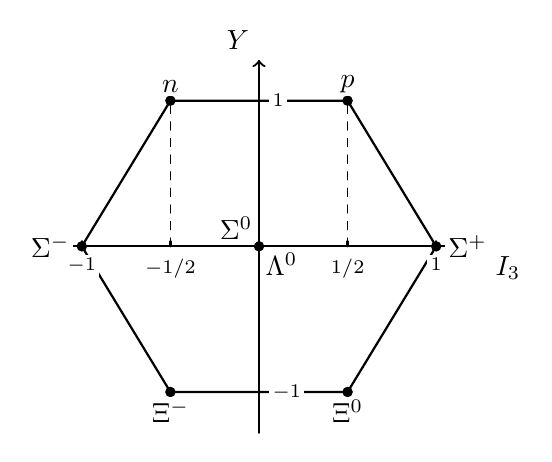
\begin{tikzpicture}[x=2.25cm,y=1.85cm, line cap=round, line join=round]

% 坐标轴
\draw[->,thick] (-1.28,0) -- (1.28,0) node[axlab,below right=2pt] {$I_3$};
\draw[->,thick] (0,-1.28) -- (0,1.28) node[axlab,above left=2pt] {$Y$};

% 八重态点
\coordinate (Sigm-) at (-1,0);
\coordinate (Sigm0) at (0,0);
\coordinate (Sigm+) at (1,0);

\coordinate (n) at (-0.5,1);
\coordinate (p) at ( 0.5,1);

\coordinate (xim) at (-0.5,-1);
\coordinate (xi0) at ( 0.5,-1);

% 外边六边形
\draw[thick] (Sigm-) -- (n) -- (p) -- (Sigm+) -- (xi0) -- (xim) -- cycle;

% 实心点
\foreach \P in {Sigm-,n,p,Sigm+,xi0,xim,Sigm0}
  \fill (\P) circle (1.9pt);

% 两条虚线
\draw[dashed] (-0.5,0) -- (-0.5,1);
\draw[dashed] ( 0.5,0) -- ( 0.5,1);

% 粒子标注）
\node[plab,above=1.5pt]      at (n) {$n$};
\node[plab,above=1.5pt]      at (p) {$p$};

\node[plab,left=3pt]         at (Sigm-) {$\Sigma^-$};
\node[plab,right=3pt]        at (Sigm+) {$\Sigma^+$};

% 中心两态
\node[plab,above left=1pt]   at (Sigm0) {$\Sigma^0$};
\node[plab,below right=1pt]  at (Sigm0) {$\Lambda^0$};

\node[plab,below=1.5pt]      at (xim) {$\Xi^-$};
\node[plab,below=1.5pt]      at (xi0) {$\Xi^0$};

% 刻度线
\foreach \x in {-1,-0.5,0.5,1}  \draw[thick] (\x,0) -- (\x,0.035);
\foreach \y in {-1,1}          \draw[thick] (0,\y) -- (0.035,\y);

% x 轴刻度数字
\node[ticklab,below=3pt] at (-1,0)   {$-1$};
\node[ticklab,below=3pt] at (-0.5,0) {$-1/2$};
\node[ticklab,below=3pt] at ( 0.5,0) {$1/2$};
\node[ticklab,below=3pt] at ( 1,0)   {$1$};

% y 轴刻度数字
\node[ticklab,right=3.5pt] at (0, 1) {$1$};
\node[ticklab,right=3.5pt] at (0,-1) {$-1$};

\end{tikzpicture}
\end{minipage}
\hfill
%==============================================================
%重子十重态
%==============================================================
\begin{minipage}{0.48\textwidth}
\centering
\begin{tikzpicture}[x=2.05cm,y=1.65cm, line cap=round, line join=round]

% 坐标轴
\draw[->,thick] (-1.75,0) -- (1.75,0) node[axlab,below right=2pt] {$I_3$};
\draw[->,thick] (0,-2.25) -- (0,1.35) node[axlab,above left=2pt] {$Y$};

% 十重态关键坐标）
\coordinate (Dm)   at (-1.5, 1);   % Delta-
\coordinate (D0)   at (-0.5, 1);   % Delta0
\coordinate (Dp)   at ( 0.5, 1);   % Delta+
\coordinate (Dpp)  at ( 1.5, 1);   % Delta++

\coordinate (Ssm)  at (-1, 0);     % Sigma*-
\coordinate (Ss0)  at ( 0, 0);     % Sigma*0
\coordinate (Ssp)  at ( 1, 0);     % Sigma*+

\coordinate (Xsm)  at (-0.5,-1);   % Xi*-
\coordinate (Xs0)  at ( 0.5,-1);   % Xi*0

\coordinate (Om)   at ( 0,-2);     % Omega-

% 外三角形边
\draw[thick] (Dm) -- (Om) -- (Dpp) -- cycle;

% 顶边与内层水平线
\draw[thick] (Dm) -- (Dpp);              % Y=1 顶边
\draw[thick] (Xsm) -- (Xs0);             % Y=-1 内水平线

% 用“短竖划”标记各态位置
% 顶边上的 Δ^0,Δ^+ 位置短划
\draw[thick] ($(D0)+(0,0.05)$) -- ($(D0)+(0,-0.05)$);
\draw[thick] ($(Dp)+(0,0.05)$) -- ($(Dp)+(0,-0.05)$);
% I3 轴上的 Σ* 三态短划
\foreach \P in {Ssm,Ss0,Ssp}{
  \draw[thick] ($(\P)+(0,0.05)$) -- ($(\P)+(0,-0.05)$);
}
% Y=-1 线上 Ξ* 两态短划
\foreach \P in {Xsm,Xs0}{
  \draw[thick] ($(\P)+(0,0.05)$) -- ($(\P)+(0,-0.05)$);
}

% 粒子标注
\node[plab,above left=1pt]  at (Dm)  {$\Delta^-$};
\node[plab,above=1.5pt]     at (D0)  {$\Delta^0$};
\node[plab,above=1.5pt]     at (Dp)  {$\Delta^+$};
\node[plab,above right=1pt] at (Dpp) {$\Delta^{++}$};

\node[plab,above=2pt] at (Ssm) {$\Sigma^{*-}$};
\node[plab,above=2pt] at (Ss0) {$\Sigma^{*0}$};
\node[plab,above=2pt] at (Ssp) {$\Sigma^{*+}$};

\node[plab,left=3pt]  at (Xsm) {$\Xi^{*-}$};
\node[plab,right=3pt] at (Xs0) {$\Xi^{*0}$};

\node[plab,left=3pt] at (Om)  {$\Omega^-$};

% 坐标轴刻度线
\foreach \x in {-1.5,-1,-0.5,0.5,1,1.5} \draw[thick] (\x,0) -- (\x,0.04);
\foreach \y in {1,-1,-2}                \draw[thick] (0,\y) -- (0.04,\y);

% x 轴刻度数字
\node[ticklab,below=3pt] at (-1.5,0) {$-3/2$};
\node[ticklab,below=3pt] at (-1,0)   {$-1$};
\node[ticklab,below=3pt] at (-0.5,0) {$-1/2$};
\node[ticklab,below=3pt] at ( 0,0)   {$0$};
\node[ticklab,below=3pt] at ( 0.5,0) {$1/2$};
\node[ticklab,below=3pt] at ( 1,0)   {$1$};
\node[ticklab,below=3pt] at ( 1.5,0) {$3/2$};

% y 轴刻度数字
\node[ticklab,right=3.5pt] at (0, 1)  {$1$};
\node[ticklab,right=3.5pt] at (0,-1)  {$-1$};
\node[ticklab,right=3.5pt] at (0,-2)  {$-2$};

\end{tikzpicture}
\end{minipage}

\caption{ \((1/2)^+\) 与 \((3/2)^+\) 重子的权图（横轴为同位旋第三分量 \(I_3\)，纵轴为超荷 \(Y\)）。}
\label{fig:baryon_weight_diagrams}
\end{figure}

基态重子八重态为$J^P = \frac{1}{2}^+$,可以表示为
\begin{equation}
    B = \begin{pmatrix}
    \frac{\Sigma^0}{\sqrt{2}} + \frac{\Lambda^0}{\sqrt{6}} & \Sigma^+ & p \\
    \Sigma^- & -\frac{\Sigma^0}{\sqrt{2}} + \frac{\Lambda^0}{\sqrt{6}} & n \\
    \Xi^- & \Xi^0 & -\frac{2\Lambda}{\sqrt{6}}
    \end{pmatrix} ,
\end{equation}
目前实验观测的结果表明，质子的质量$(m_p=939.27\,\text{MeV})$和中子的质量$(m_n=939.57\,\text{MeV})$非常接近，且它们的电荷分别为$+1$和$0$，这与它们的夸克组成（$uud$和$udd$）以及相应的量子数完全一致。这些实验结果强烈支持了传统夸克模型对于基态重子八重态结构的描述。
而基态重子十重态为$J^P = \frac{3}{2}^+$:
%其中$\Delta$态为$uuu$、$uud$、$udd$、$ddd$四种组合，$\Sigma^*$态为$uus$、$uds$、$dds$三种组合，$\Xi^*$态为$uss$、$dss$两种组合，而$\Omega^-$态则是由三个$s$夸克组成的。
\begin{equation}
\begin{aligned}
\Omega^- &= sss, \qquad 
\Xi^{*0} = \frac{1}{\sqrt{3}}\left(uss + sus + ssu\right), \qquad
\Xi^{*-} = \frac{1}{\sqrt{3}}\left(dss + sds + ssd\right), \\[6pt]
\Sigma^{*+} &= \frac{1}{\sqrt{3}}\left(suu + usu + uus\right), \qquad
\Sigma^{*-} = \frac{1}{\sqrt{3}}\left(sdd + dsd + dds\right), \\[6pt]
\Sigma^{*0} &= \frac{1}{\sqrt{6}}\left(sud + dsu + uds + sdu + dus + usd\right), 
\qquad
\Delta^{++} = uuu, \\[6pt]
\Delta^{+} &= \frac{1}{\sqrt{3}}\left(uud + udu + duu\right), \qquad
\Delta^{0} = \frac{1}{\sqrt{3}}\left(udd + dud + ddu\right), \qquad
\Delta^{-} = ddd .
\end{aligned}
\end{equation}


\section{奇特强子态及其非微扰研究方法}
虽然传统的夸克模型在描述强子结构方面取得了巨大成功，但它也并不是绝对正确的。随着实验的一步步深入，除了传统的$qqq$重子和$q\bar{q}$介子之外，越来越多的其他类型的强子态被发现，不同于传统意义上的色单态，它们的结构更为复杂，包括混杂态、胶子球、四夸克态$qq\bar{q}\bar{q}$、五夸克态$qqqq\bar{q}$、介子-介子分子态$((q\bar{q})(q\bar{q}))$和介子-重子分子态$((q\bar{q})(q\bar{q}))$，这些态被统称为奇特强子态。
它们既包括出现在隐粲/隐底能区的 $XYZ$ 态与带电的 $Z$ 态，其带电性直接表明其至少含有四个价夸克成分，也包括在 $\Lambda_b$ 等重味强子弱衰变的振幅分析中出现的五夸克候选结构。
值得强调的是，许多候选态的质量位置与特定强子对阈值高度接近，使得耦合道动力学、重散射效应与近阈值极点结构在其形成中可能扮演关键角色；因此，当前研究的核心主要是这些结构在解析延拓下是否存在对应 $S$ 矩阵极点、其量子数与衰变动力学是否一致、以及其内部结构究竟更接近弱束缚的强子分子态、紧致多夸克束缚态还是混杂态.\\

鉴于量子色动力学（QCD）具有渐近自由的性质，当相互作用过程具有较大的动量转移时，强相互作用耦合常数 $\alpha_s$ 变得较小，此时可以通过微扰展开对理论进行系统计算，这一理论框架通常称为微扰量子色动力学（PQCD）。微扰QCD在描述深度非弹性散射、高能强子产生以及重味产生等高能过程方面取得了显著成功。

然而，在典型的强子能标下，强子的能量尺度通常只有几个 $\mathrm{GeV}$。在这一能区，强耦合常数 $\alpha_s$ 不再是小参数，而是接近甚至大于 $1$，从而使得微扰展开方法失效。同时，由于QCD的非阿贝尔规范结构，其动力学方程具有高度非线性，目前尚无法对完整的非微扰量子色动力学进行严格解析求解。因此，在研究强子结构与强子相互作用等低能强子物理问题时，必须依赖一系列非微扰方法和有效理论框架。

目前常用的非微扰QCD研究方法主要包括格点QCD计算、QCD求和规则方法、组分夸克模型以及Dyson--Schwinger$(D-S)$方程方法等。此外，在低能区域还广泛采用有效场论的思想来描述强子之间的相互作用，例如手征微扰理论和手征有效场论等。这些方法从不同角度对非微扰强相互作用进行了刻画，为理解强子谱结构以及奇特强子态的性质提供了重要的理论工具。\\

格点量子色动力学通过在离散的时空格点上建立QCD理论，从而能够在夸克和胶子的基本自由度层面同时处理微扰与非微扰效应，并利用蒙特卡罗方法进行数值计算得到物理量。该方法在计算强子基态性质方面取得了显著成功，例如能够较为准确地给出强子质量谱以及一些重要的非微扰参数。近年来，格点QCD的计算精度不断提高，在强子结构与强子谱研究中发挥着重要作用。然而，由于计算规模巨大，对计算资源的需求极高，目前在更复杂体系中的应用仍然受到一定限制。

另一种重要的非微扰方法是QCD求和规则。在这一方法中，强子通过具有相同量子数的插值流来描述，并通过构造两点或多点关联函数，将强子性质与QCD真空凝聚参数联系起来。通过算符乘积展开与色散关系，可以从QCD层面提取强子的质量与耦合常数等物理量。尽管QCD求和规则在强子谱研究中取得了广泛应用，但由于需要对高维算符和连续谱部分进行近似处理，其计算结果通常具有一定的不确定性。

组分夸克模型则将组分夸克视为有效自由度，通过引入夸克之间的有效相互作用势来描述强子的结构与谱性质。该模型在解释低能强子谱和强子间相互作用方面取得了较大成功，并在直观理解强子结构方面具有重要意义。然而，由于模型本身并非直接从QCD基本方程严格推导得到，因此在描述强相互作用的非微扰动力学方面仍然存在一定局限。

Dyson--Schwinger 方程方法则提供了一种从场论角度研究非微扰QCD的连续方法。该方法通过建立格林函数之间的自洽方程组，将 $n$ 点格林函数与更高阶的格林函数联系起来，从而形成一组无限耦合的Dyson--Schwinger方程。理论上，如果能够完整求解这一方程组，则可以严格描述QCD的全部动力学性质。然而在实际计算中必须对方程组进行适当截断并引入合理的近似，因此其结果仍依赖于具体的截断方案。尽管如此，该方法在研究强子结构、手征对称性破缺以及夸克传播子性质等问题上取得了重要进展。

总体而言，这些理论方法从不同角度刻画了QCD的非微扰动力学，为研究强子结构、强子谱以及奇特强子态提供了重要的理论工具，同时也在各自的适用范围内存在一定的局限性。\\

在低能强子物理研究中，另一类重要的理论工具是有效场论方法。有效场论的基本思想是利用体系在特定能标下的有效自由度来构建理论，从而在不需要完整求解QCD基本方程的情况下描述强相互作用的动力学性质。在低能区域，QCD 的手征对称性及其自发破缺起着决定性作用，因此可以以轻赝标介子作为有效自由度构建手征有效理论。基于这一思想建立的手征微扰理论为研究低能强子相互作用提供了系统的展开框架，并能够在动量或轻夸克质量的幂级数展开下给出可计算的相互作用振幅。

然而，手征微扰理论本质上是一种微扰展开方法，其适用范围主要局限于低能区域。当能量接近共振区时，简单的微扰展开往往无法描述强子散射振幅中的共振结构。为了克服这一问题，人们在手征有效理论的基础上引入幺正化方法，从而发展出手征幺正方法。该方法首先由手征有效拉氏量得到强子之间的相互作用势，然后通过求解散射方程实现振幅的幺正化处理，使得得到的散射矩阵满足幺正条件。在这一框架下，强子共振可以作为散射振幅在复能量平面上的极点自然产生，因此许多共振态可以被解释为由强子之间的动力学相互作用生成的态。

在手征幺正方法中，强子之间的相互作用首先由手征微扰理论最低阶手征拉氏量给出，从而得到相互作用势 $V$。随后通过求解动力学的 Bethe--Salpeter 方程对散射振幅进行幺正化处理，使得到的散射矩阵满足幺正条件。
手征幺正方法同时结合了QCD低能区域的手征对称性约束与散射矩阵的幺正性条件，因此能够在耦合道相互作用中自然地产生共振结构。在这一框架下，一些强子共振并不需要作为基本自由度引入，而是可以由不同强子道之间的动力学相互作用生成，其物理图像通常被解释为强子分子态。

与传统的有效模型相比，手征幺正方法通过求解散射方程在理论上等价于对无穷级圈图进行求和，因此能够在非微扰水平上描述强子相互作用。整个理论框架中自由参数较少，其主要来源于传播子圈函数 $G$ 的重整化过程。在常用的三动量截断重整化方案中，唯一的重要参数为截断动量 $q_{\text{max}}$，该参数反映了动量空间中有效相互作用的范围。

截断动量 $q_{\text{max}}$ 的大小通常通过拟合实验中已知共振态的极点位置来确定。当该参数被固定之后，理论模型便具有一定的预测能力，可以进一步用于研究相关体系中的散射过程以及一系列奇特强子态的质量、宽度和耦合常数等性质。因此，手征幺正方法在近年来的强子谱学研究中得到了广泛应用，并成为研究奇特强子态结构的重要理论工具。\\

手征幺正方法在研究轻强子与重味强子体系中都取得了广泛成功。例如，在介子–介子以及介子–重子散射中，该方法能够自然产生一系列已知的共振态，并对其质量、宽度以及耦合常数给出合理描述。特别是在多耦合道体系中，幺正化处理能够有效考虑不同散射道之间的耦合效应，从而在理论上再现实验观测到的共振结构。因此，手征幺正方法已成为研究强子谱结构、强子相互作用以及奇特强子态形成机制的重要理论工具之一。


